\section{Results}

Compare all the methods in a table in order to show the performance.

Comment on the amount of dimensions vs errors.


\begin{table}[H]
\centering
\begin{tabular}{llllll}
\hline
Class		&	Linear	&  Discriminative  & GMM  & ANN	& SVM \\ \hline
Nicolai Error &	24.91\%  & 24.27\%  &  9.06\%  & 10.35\%  &  3.56\% \\
Rasmus Error  &	11.00\%  & 10.68\%  & 21.68\%  & 10.03\%  & 24.92\% \\
Rune Error	  &	30.74\%  & 29.77\%  & 16.18\%  & 16.82\%  & 36.57\% \\ \hline
Total Error	  &	22.22\%  & 21.58\%  & 15.64\%  & 12.41\%  & 21.68\% \\ \hline
\end{tabular}
\caption{ Error of test data }
\end{table}



\begin{table}[H]
\centering
\begin{tabular}{llllll}
\hline
Class		&	Linear	&  Discriminative  & GMM  & ANN	& SVM \\ \hline
Nicolai Error &	14.76\%  & 10.34\%  &  0.41\%  & 0\%  &  0\% \\
Rasmus Error  &	10.48\%  & 11.59\%  & 0.14\%  & 0\%  & 0\% \\
Rune Error	  &	23.17\%  & 18.48\%  & 2.06\%  & 0\%  & 0\% \\ \hline
Total Error	  &	16.14\%  & 13.47\%  & 0.87\%  & 0\%  & 0\% \\ \hline
\end{tabular}
\caption{ Error of training data }
\end{table}


\begin{figure}[H]
\centering
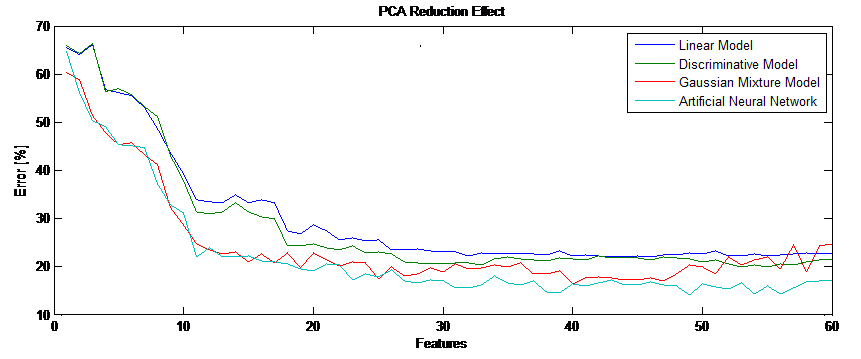
\includegraphics[scale=0.7]{billeder/PCAReductionEffect}
\caption{ Dimensions effect on Error }
\label{fig:DimError}
\end{figure}

%------------------------------------------------
